\documentclass[10pt]{article}
\usepackage[polish]{babel}
\usepackage[utf8]{inputenc}
\usepackage[T1]{fontenc}
\usepackage{amsmath}
\usepackage{amsfonts}
\usepackage{amssymb}
\usepackage[version=4]{mhchem}
\usepackage{stmaryrd}
\usepackage{graphicx}
\usepackage[export]{adjustbox}
\graphicspath{ {./images/} }

\title{LIGA MATEMATYCZNA im. Zdzisława Matuskiego \\
 FINAE \\
 24 kwietnia 2017 \\
 SZKOŁA PONADGIMNAZJALNA }

\author{}
\date{}


\begin{document}
\maketitle
\section*{ZADANIE 1.}
Dane są dwie bliźniacze (to znaczy różniące się o 2) liczby pierwsze. Udowodnij, że nie mogą one być przyprostokątnymi trójkąta prostokątnego o wszystkich bokach o długości całkowitej.

\section*{ZADANIE 2.}
Na tablicy napisano dwie liczby: pierwszą i drugą. Następnie napisano liczbę trzecią, która jest sumą pierwszej i drugiej, potem zapisano czwartą liczbę, która jest sumą drugiej i trzeciej. I tak dalej aż do dziesiątej liczby. Suma wszystkich dziesięciu liczb napisanych na tablicy jest równa 5005. Wyznacz siódmą liczbę.

\section*{ZADANIE 3.}
Czy liczbę 1 można przedstawić jako sumę ułamków \(\frac{1}{a}, \frac{1}{b}, \frac{1}{c}, \frac{1}{d}\), gdzie \(a, b, c, d\) są nieparzystymi liczbami naturalnymi?

\section*{ZADANIE 4.}
Danych jest 21 liczb rzeczywistych. Wiadomo, że suma każdych jedenastu spośród tych liczb jest większa od sumy pozostałych dziesięciu. Wykaż, że wszystkie liczby są dodatnie.

\section*{ZADANIE 5.}
Oblicz pole trapezu prostokątnego wiedząc, że odległości środka okręgu wpisanego w ten trapez od końców ramienia nieprostopadłego do podstaw, są równe \(a\) oraz \(2 a\).

\section*{ZADANIE 6.}
W zbiorze liczb rzeczywistych rozwiąż układ równań

\[
\left\{\begin{array}{l}
x^{2}+9=4 y \\
y^{2}+1=6 z \\
z^{2}+4=2 x
\end{array}\right.
\]

\section*{ZADANIE 7.}
Czworokąt \(A B C D\) jest wpisany w okrąg. Proste \(A B\) i \(C D\) przecinają się w punkcie \(E\), a proste \(A D\) i \(B C\) przecinają się w punkcie \(F\). Udowodnij, że jeśli \(|B E|=|D F|\), to \(|C E|=|C F|\).\\
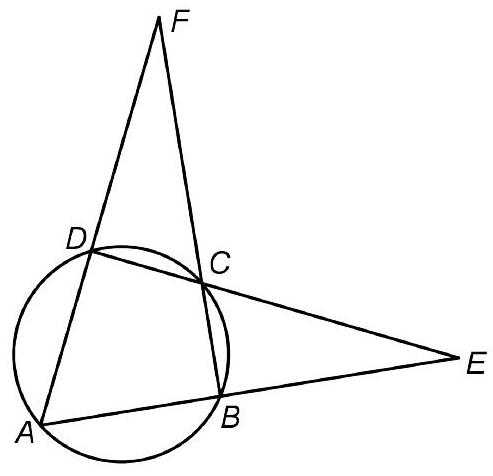
\includegraphics[max width=\textwidth, center]{2024_11_21_5f95dfee814a2786343ag-1}


\end{document}